\documentclass{llncs}

\usepackage{listings}
\usepackage[export]{adjustbox}

\lstdefinelanguage{Coq}{
  ,morekeywords={match,end,Definition,Inductive,Lemma,Record,
    Variable,Section,case,of,if,then,else,is,let,in,do,return,with}%
  ,keywordstyle=\bfseries
  ,basicstyle=\sffamily
  ,columns=fullflexible
  ,numberstyle=\tiny
  ,escapeinside={@}{@}
  ,literate=
  {<-}{{$\leftarrow\;$}}1
  {=>}{{$\rightarrow\;$}}1
  {->}{{$\rightarrow\;$}}1
  {<->}{{$\leftrightarrow\;$}}1
  {<==}{{$\leq\;$}}1
  {\\/}{{$\vee\;$}}1
  {/\\}{{$\land\;$}}1
}
\lstset{language=Coq}

\begin{document}

\title{Monte Carlo: Estimation of Pi}

\author{Jacob Mulligan}
\institute{Ohio University, Athens, OH 45701}

\maketitle

\section{Introduction}

\subsection{Subsection1} 	For my final Project I chose to do the Monte Carlo estimation of pi. I’m sure most are aware of Pi and that it is an irrational number and an extremely important mathematical constant in many applications of applied science. Pi was initially called Archimedes constant, because it was discovered by Archimedes using a circle and multiple polygons. Starting with a hexagon and eventually working his way up to a 96-sided polygon. How this works is from the ratio of:
\begin{equation}
Pi = Circumference(perimeter)/Diameter.
\end{equation}
Continually increasing the sides, the approximation gets closer however, too many sides and the estimation becomes too high for the expected value. After all of Archimedes’ calculations his estimation of pi came out as:
\begin{equation}
3.14084 < pi < 3.14285
\end{equation}
Individually the lower and upper bound of the inequality yields a percent error of 0.023873261628667\% error for the lower and 0.040107079536167\% error for the upper. They are close estimations and Archimedes is no doubt a genius of his time for figuring this out, but there are newer approaches to get the estimation of pi and the method I used for my final project yielded a much lower percent error comparing it to the expected value. 
I have always had an interest in the value pi because of its countless applications in math and science. I also find it interesting how there are multiple ways in calculating its value.\\

\subsection{Subsection2} In my project I use a Monte Carlo method in estimating the value of pi. A Monte Carlo Method is when simulations are used to model the probability of different outcomes in a process that cannot easily be predicted due to the intervention of random variables. It is a technique used in most fields to understand the impact of risk and uncertainty in prediction and forecasting models. However,what makes my work interesting compared to existing methods of the Monte Carlo estimation of pi is that my method runs a Monte Carlo simulation on Monte Carlo simulations. This approach I found best and most interesting because it yielded better results meaning a closer estimation of the expected value, opposed to running a singular Monte Carlo simulation.

\section{Technical Development}
\subsection{Subsection1}At the beginning the project presents the method to which the estimation of pi can be determined. Suppose you have a circle inscribed in a square. The experiment simply consists of throwing darts on this figure completely at random (meaning that every point on the dartboard has an equal chance of being hit by the dart). How can we use this experiment to estimate Pi? The platform of the experiment will look something like this.\\
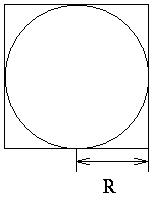
\includegraphics[width=0.4\textwidth, center]{squarecircle}
The answer can be determined by using geometry and the statistical outcome of throwing the darts. If we let the radius of the circle be R then the area of the circle will be equal to Pi R2 and the area of the square will be equal to 4R2. Now if one divides the area of the circle by the area of the square, we get Pi/4. However, this still doesn’t give the answer to our question. This only gives us the Probability distribution of:
\begin{equation}
P (point inside circle) = Pi/4 
\end{equation}
\\
So, how do we get Pi by the simulation?  In our case for the simulation we are randomly throwing darts at this shape and all of the darts will land within the square, but not all of them will land inside of the circle. So, if we are truly throwing at random this experiment will estimate the ratio of the area of the circle to the area of the square, by counting the number of points that fall in each the square and the circle. From our geometry ration we got Pi/4 so now we can estimate Pi using this equation:
\begin{equation}
Pi = 4 * (number of points in circle) / (number of points in square)
\end{equation}
This gives us all we need to create the Monte Carlo simulation and in code it will look something like this as well as a visual of what the square and circle will look like as well:\\
\begin{lstlisting}
import random as r
import math as m

inside = 0

total = 100000
limit = 10

# Iterate for the number of darts.
for i in range(0, total):
# Generate random x, y in [0, 1].
    x2 = r.random()**2
    y2 = r.random()**2
        # Increment if inside unit circle.
    if m.sqrt(x2 + y2) < 1.0:
        inside += 1

# inside / total = pi / 4
pi = (float(inside) / total) * 4

# It works!
print("First experimental pi value")
print(pi)

\end{lstlisting}
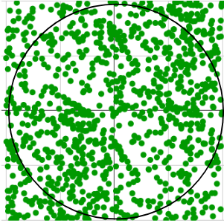
\includegraphics[width=0.4\textwidth, center]{simulatedPi} \newline
This single simulation yields an estimation of 3.1672 with a percent error of 0.8151281261220308\% when compared to the expected value of 3.141592. An interesting thing about Monte Carlo simulations is that the more data you have the more accurate. If I change the simulation to run over 10,000,000 points versus the initial 100,000 points the simulation results in an estimation of 3.1421332 and a percent error of 0.017226934624222284\%. It is obvious that the increased amount of points gets a closer estimation of Pi however, I wanted to get closer using the same amount of points.\\
The approach I took to get a closer estimation was to run a Monte Carlo simulation of my Monte Carlo simulation. So, I took the single simulation above and repeated it 9 times each running over 10,000,000 random points. Keeping track of each simulations estimation I took the average of them together, and from that average I compared it to the expected value of Pi to get the percent error of my experiment. In addition to that I wanted to compare the results of the different applied methods, So I also found the percent difference comparing two of my experimental estimations of Pi. The following is some of the highlights from my code to demonstrate what I am talking about.\\
\begin{lstlisting}
print("average experimental value from all simulations")
avg = float((pi + pi2 + pi3 + pi4 + pi5 + pi6 + pi7 + pi8 + pi9)/9)
print(avg)

abavg = abs(avg - expected)
error = float(abavg / expected) * 100
print("average experimental value percent error")
print(error)

print("The percent difference between the two experimental values")
upper = abs(pi - avg)
lower = (float(pi + avg))/2
diff = (upper/lower)*100
print(diff)    
\end{lstlisting}

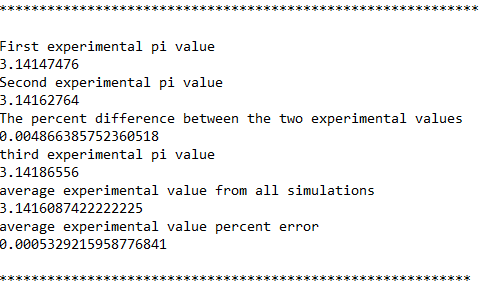
\includegraphics[width=1\textwidth, center]{dataimage2}
The above data is the results of running the simulation as well as some additional statistical analysis. As you can see the estimation of Pi shows a much lower percent error compared to running the simulation only one time over the same number of random draws. Thus, one can see that the Monte Carlo method proves to be an accurate way to determine a close estimation of Pi.\\


\section{Conclusion}One general lesson that can be learned bout this experiment is the value in comparing the methods used. It’s important to distinguish which method shows the best results even though both are correct. The purpose of Monte Carlo simulations is not to make the decision for the user but to aid in that process by the data it provides. This makes it easy for us to be able to analyze the methods used get the wanted results.\\
Another lesson I learned from this project is the overall value of Monte Carlo simulations. The estimation of Pi is just a singular use of applying this method that can be used in so many ways. I was interested to learn that machine learning uses Monte Carlo methods to obtain data to better train their A.I. as well as investors to calculate risk on trades and stocks.\\
I think if I were to continue this project my next steps would be to try and speed up the simulation because running it 9 times over 10 million data points means that it takes a long time to get results. In conclusion I hope that my method was made clear in how I obtained my results in proving my estimation. As well as demonstrating how I was not only able to achieve the desired approximation, but also improve the results by applying my own method. 


\bibliographystyle{plain}
\bibliography{references}
“Monte Carlo Estimation for Pi.” B.U. Center for Polymer Studies:JAVA Applets, http://polymer.bu.edu/java/java/montepi/MontePi.html.\\
\\Kenton, Will. “Monte Carlo Simulation.” Investopedia, Investopedia, 18 Nov. 2019, https://www.investopedia.com/terms/m/montecarlosimulation.asp.\\
\\“Estimating the Value of Pi Using Monte Carlo.” GeeksforGeeks, 8 Feb. 2018, https://www.geeksforgeeks.org/estimating-value-pi-using-monte-carlo/.\\
\\Wicklin, Rick. “Monte Carlo Estimates of Pi and an Important Statistical Lesson.” The DO Loop, 14 Mar. 2016, https://blogs.sas.com/content/iml/2016/03/14/monte-carlo-estimates-of-pi.html.

\end{document}
